%!TEX root = ../../main.tex
\section{1D scatter curve similarity analysis}
\label{sec:1D scatter curve similarity analysis}
To increase the signal to noise ratio when processing data in SAXS, it is necessary to merge 1D intensity curves from several frames.
If the scattering for different frames is from the same molecule in the sample, then the frames will be similar i.e. the frames will overlap.
However as radiation damage progresses during the experiment, the molecules begin to aggregate, which causes the intensity curve to increase at low $q$ angles and is speculated to decrease at high $q$ angles \cite{hopkins2016quantifying}.
On the other hand, fragmentation and molecule repulsion due to protein charging, cause a decrease in scattering at low $q$ angles and an increase at high $q$ angles.
Figure~\ref{fig:1D Scatter Curves} shows the scattering profile of several SAXS frames collected from the same glucose isomerase sample.
As the dose increases, there is a clear decrease in the scattered intensity at low angles suggesting that the sample is undergoing fragmentation.
This was also observed with the glucose isomerase samples used in the study conducted by Hopkins and Thorne \cite{hopkins2016quantifying}.
Therefore it is necessary to determine the similarity between any two pairs of frames to determine which frames to merge together.
Due to the fact that a new method of assessing the similarity was published between performing experiment 1 and 2 \cite{franke2015correlation}, the analysis performed on the two sets of data and presented here are different.
This was necessary because the new version of DATCMP, the software program used to perform the similarity analysis \cite{petoukhov2012new}, does not incorporate some of its old functionality utilised in Expt 1, and the online manual describing the new features has not yet been updated.
\begin{figure}
    \centering
    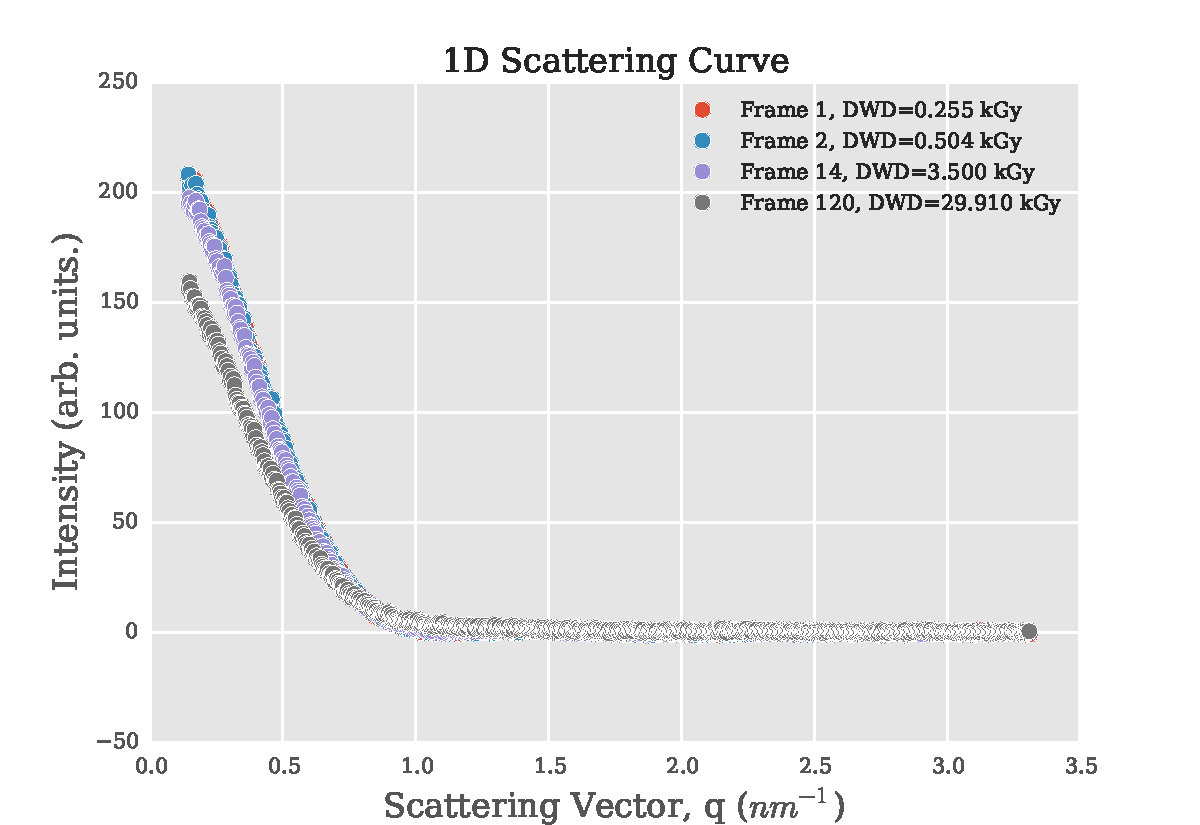
\includegraphics[width=1.0\textwidth]{figures/saxs/scatter_curves.pdf}
    \caption[Increasing dissimilarity of 1D SAXS curves with increasing X-ray exposure.]{1D scattering curves from the first run of the GI sample with no radioprotectant compounds added.
    Frames 1 and 2 visually seem to overlap well and the merging analysis determines these frames to be similar.
    Frame 14 is the first frame found to be dissimilar to frame 1.
    However, by visual inspection, the dissimilarity is not obvious.
    Frame 120 was the last frame collected in this run.
    The dissimilarity of frame 120 from the others is obvious.
    This suggests that the molecules in the sample have undergone significant radiation induced changes during the experiment.}
    \label{fig:1D Scatter Curves}
\end{figure}

\subsection{Data analysis - experiment 1}
\label{sub:Data analysis - experiment 1}
Buffer subtraction was first carried out in Sc\AA tter (Rambo, R. at DLS, Didcot, UK).
DATCROP, a utility program for cropping SAXS data, distributed as part of the ATSAS program suite \cite{petoukhov2012new}, was then used to remove data points from the very low angles around the beam stop and also from the larger angles where the signal-to-noise ratio drops considerably: this was carried out by visual inspection.
DATCMP (a program also distributed in the ATSAS suite) was then used to carry out a Scheffe \textit{post hoc} analysis on the resulting 1D scattering data (frames) for each experimental run.
This analysis compares the similarity of the first frame to each of the subsequent frames, since the first frame is produced at the lowest dose and so it is assumed to be of the best quality.
The result of the Scheffe \textit{post hoc} analysis is a `fidelity value', which is a value given for each frame to describe its similarity to the first frame.
An identical frame is given a fidelity value of 0.
Increasing fidelity values correspond to increasing dissimilarity of a particular frame from the first frame.
A plot of the fidelity values against time and diffraction weighted dose (DWD) is shown in Figure~\ref{fig:Rebecca data}.
\begin{figure}
    \ContinuedFloat
    \begin{subfigure}[b]{1.0\textwidth}
            \centering
            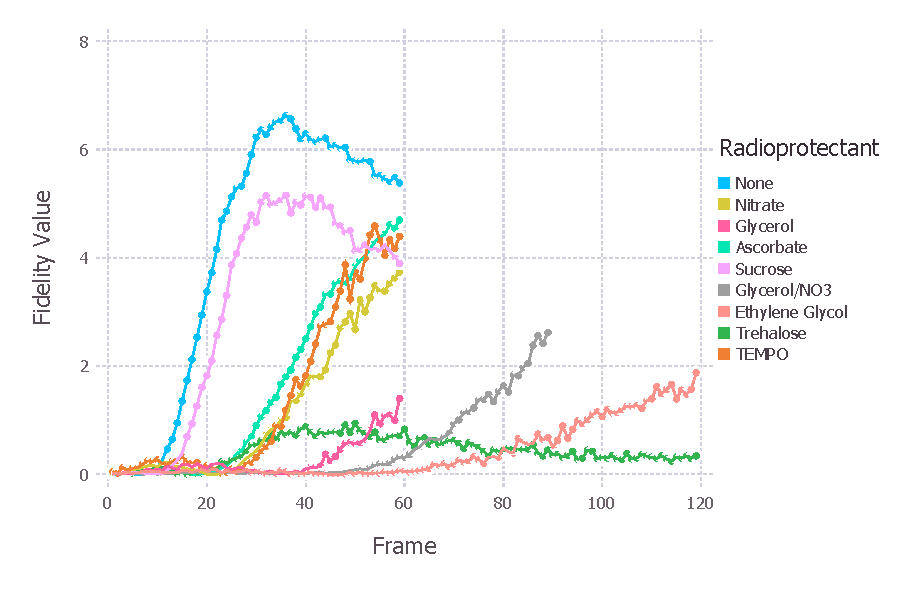
\includegraphics[width=\textwidth]{figures/saxs/cmpd_plt_frame.pdf}
            \caption{}
            \label{fig:1D scatter plot of frames 1 and 120}
    \end{subfigure}
    \\
    \begin{subfigure}[b]{1.0\textwidth}
            \centering
            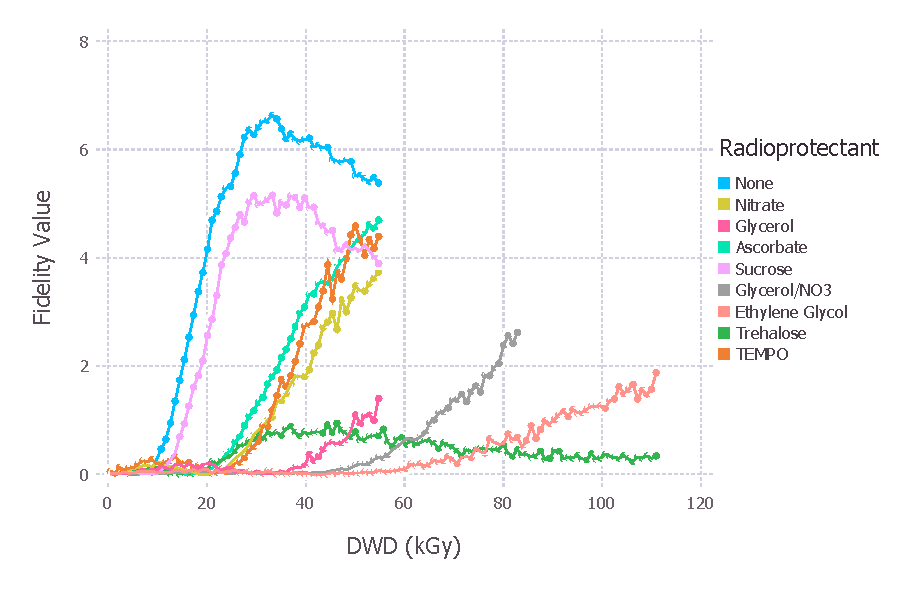
\includegraphics[width=\textwidth]{figures/saxs/cmpd_plt_dose.pdf}
            \caption{}
            \label{fig:Pairwise correlation frames 1 and 120}
    \end{subfigure}
    \caption[Fidelity value as a function of time and dose.]{(a) Fidelity value as a function of time
    (b) Fidelity value as a function of dose.
    Fidelity values start at 0 for the first frame and increase as the frames become more dissimilar.}
    \label{fig:Rebecca data}
\end{figure}
These data show the changing similarity of frames throughout the experiment, but they do not explicitly provide a quantitative metric to compare the efficacies of the various radioprotectants.
Further analysis of these data was required to achieve this.

The curves of fidelity values against both time and DWD visually resemble a logistic relationship (they look like S-shaped curves).
Thus 4-parameter logistic (4PL) functions were fitted to the data:
\begin{equation}
    F(x) = \f{a - d}{(1 + (x/c)^b)^2} + d,
    \label{eq:4PL}
\end{equation}
where $F$ is the fidelity value, $x$ is the $x$-axis coordinate (it could either be time or DWD), and $a, b, c$ and $d$ are the 4 parameters to be determined.
Each of the parameters has graphical interpretation in relation to the logistic curve.
$a$ and $d$ represent the minimum and maximum values of the curve respectively, $b$ represents the steepness of the slope and $c$ is the location of the point of inflection.
The 4PL curve was used instead of the commonly used 3 parameter logistic function (also known as the Hill function) because it allows much more flexibility for the steepness of the curve, which was likely to change with different radioprotectants.

To determine which frames should be merged it is necessary to decide on the threshold similarity criterion.
Two criteria were used:
\begin{enumerate}
    \item the DWD absorbed to reach an arbitrary value, and
    \item the DWD absorbed to reach maximum curvature of the fidelity curve.
\end{enumerate}
The first of the two criteria is straightforward to assess.
A fidelity value is chosen and then the fitted logistic function can be rearranged to find the DWD value for which the chosen fidelity value is reached.

The second of the criteria is slightly more involved. For frames to be similar, their fidelity values have to be close to zero.
Therefore the early frames should be close in value.
However when frames start to become dissimilar, the fidelity value increases.
In terms of the fitted logistic curve, this corresponds to an increasing gradient as the fidelity values increase.
The required value is the total absorbed dose at the point when the increase in the gradient of the fidelity values reaches a maximum.
To perform this analysis it was necessary to calculate the curvature, $\kappa$, of the logistic curves, which is  given by:
\begin{equation}
    \kappa(x) = \f{\f{\mathrm{d}^2F}{\mathrm{d}x^2}}{\left( 1 + \f{\mathrm{d}F}{\mathrm{d}x}\right)^{3/2}}.
    \label{eq:Curvature}
\end{equation}
This equation was calculated symbolically using the symbolic math toolbox in MATLAB. The maximum of this function was found using the MATLAB function `fminbnd' to find the minimum value of $-\kappa(x)$ i.e. the problem was converted from trying to find the maximum into a problem in which the same solution is found by finding the minimum. This is a common procedure for optimisation problems.

An implicit assumption with the methods described is that damage is entirely progressive and subsequent frames beyond the threshold are all significantly dissimilar.
Mathematically this assumption manifests itself as logistic functions representing the fidelity as a monotonically increasing function of the dose.

\subsection{Data analysis - experiment 2}
\label{sub:Data analysis - experiment 2}
In a similar manner to the analysis performed on the results from Expt 1, buffer subtraction and cropping was performed before 1D curve similarity analysis.
However these steps were performed with custom written Python scripts.
This was done for two reasons:
the first was that the pipeline could then be completely scripted (Sc\AA tter, which was used for buffer subtraction for data processing for Expt 1, is a GUI based program written in Java),
and secondly, DATCROP subtracts data from files, so the scripts that were written would require many file handling operations, which are relatively time consuming computationally.
Therefore writing the scripts to perform these simple operations (subtraction and cropping) was much more time efficient and allowed for more flexibility.

DATCMP was again used for the similarity analysis.
However, as mentioned in section \ref{sec:1D scatter curve similarity analysis}, the method used in the current version has been changed by the authors of this software since the Expt 1 analysis.
The new method is called the Correlation Map (CorMap) test \cite{franke2015correlation}.
Unlike the algorithm used to generate the fidelity values, the CorMap test does not require any estimates of the experimental errors to test similarity.

A full explanation of the method can be found in Franke \textit{et al.} (2015), but the main ideas are presented here and tested for their suitability for application to our data.
Any two frames can be compared using a pairwise correlation, which involves calculating the difference between the two intensity curves.
If the two frames are identical up to the noise level, then the difference between them is a random number.
Given that the intensity values are assumed to come from a normal distribution \cite{franke2015correlation}, the difference between them is normally distributed with a mean of zero.
Due to the symmetry of the normal distribution, the probability of the difference of the data being either positive or negative is 0.5.
The pairwise CorMaps between selected frames from the experiment are shown in Figure~\ref{fig:Pairwise correlation plots}.
Notice that for similar frames 1 and 2 (Figure~\ref{fig:1D scatter plot of frames 1 and 2}), the pairwise CorMap resembles a randomised lattice (Figure~\ref{fig:Pairwise correlation frames 1 and 2}) as expected for identical data.
Conversely, for dissimilar frames 1 and 120 (Figure~\ref{fig:1D scatter plot of frames 1 and 120}), the pairwise CorMap shows large regions of white and black patches, suggesting that the frames are systematically different.
DATCMP performs quantitative analysis that formalises the similarity conclusions that can be drawn from these CorMaps.
\begin{figure}
    \centering
    \begin{subfigure}[b]{0.9\textwidth}
            \centering
            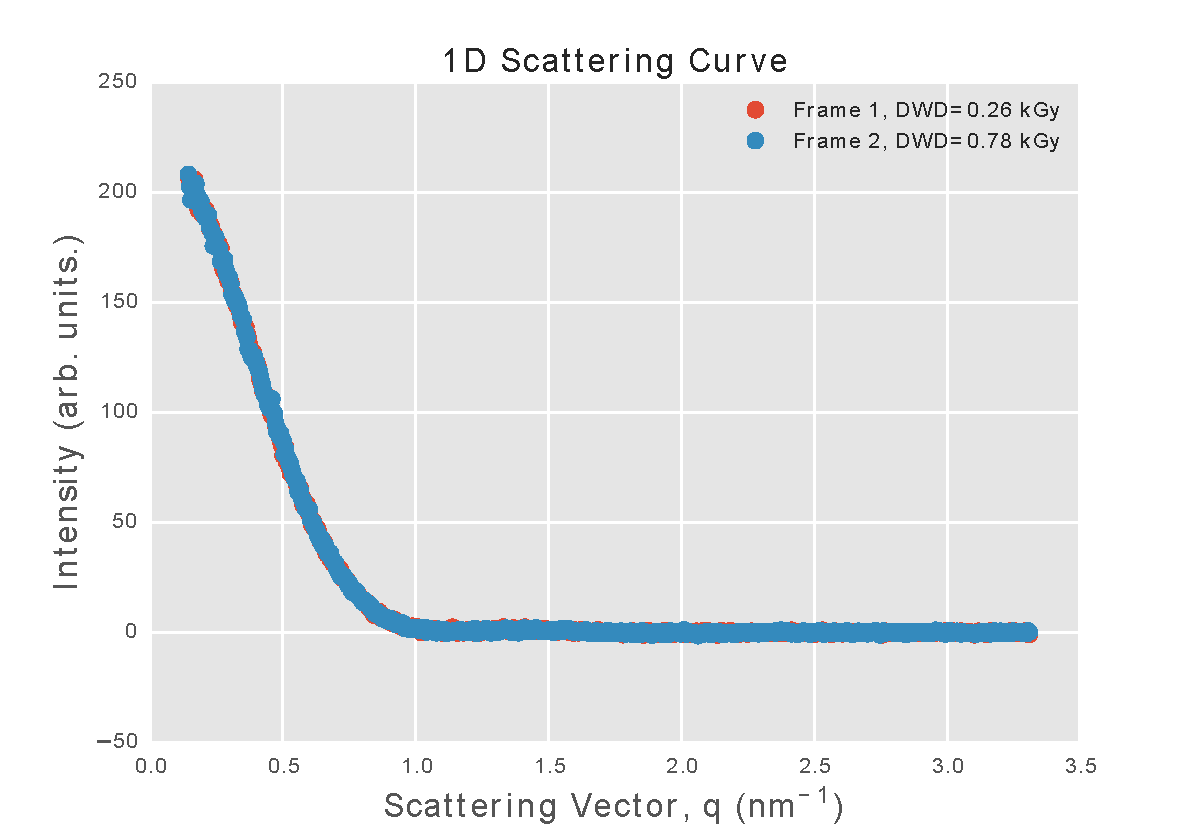
\includegraphics[width=\textwidth]{figures/saxs/scatter_curve_frames_1_2_amended.pdf}
            \caption{}
            \label{fig:1D scatter plot of frames 1 and 2}
    \end{subfigure}
    \\
    \begin{subfigure}[b]{0.9\textwidth}
            \centering
            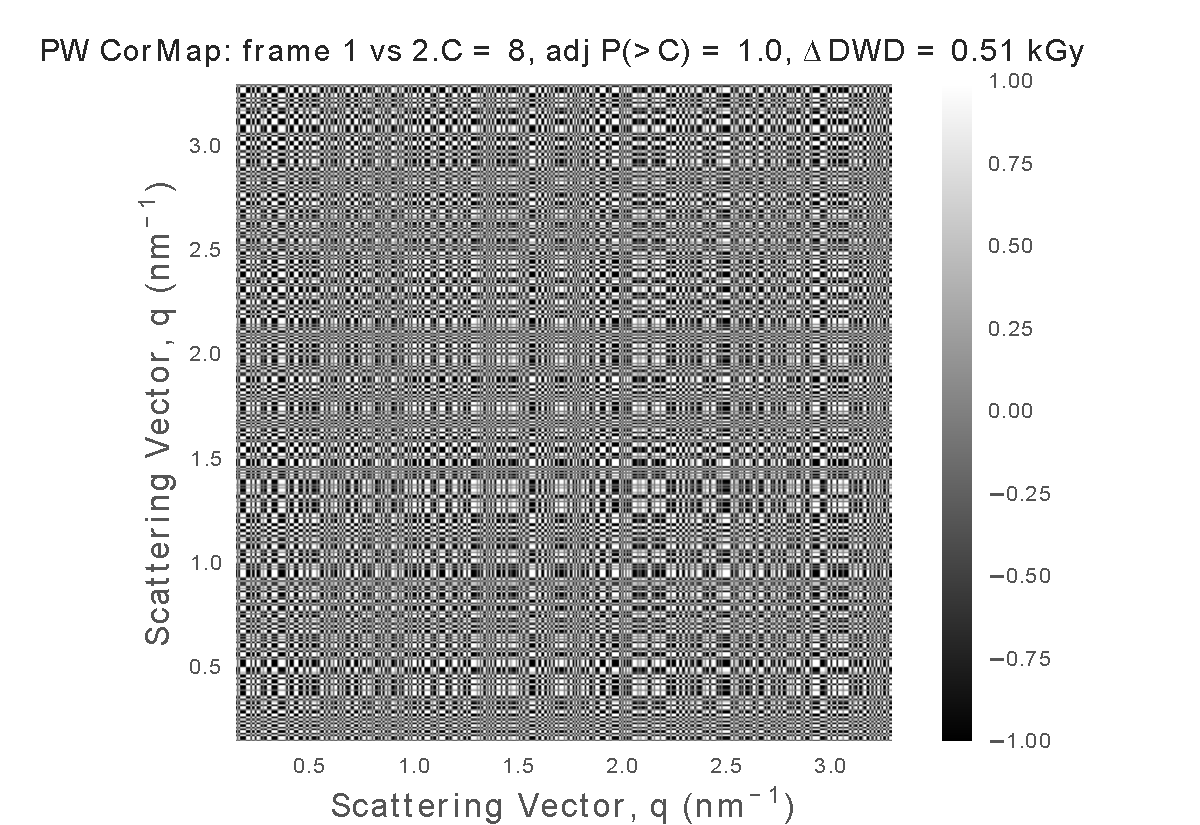
\includegraphics[width=\textwidth]{figures/saxs/pwcormap_frames_1_2_amended.pdf}
            \caption{}
            \label{fig:Pairwise correlation frames 1 and 2}
    \end{subfigure}
\end{figure}
\begin{figure}
    \ContinuedFloat
    \begin{subfigure}[b]{0.9\textwidth}
            \centering
            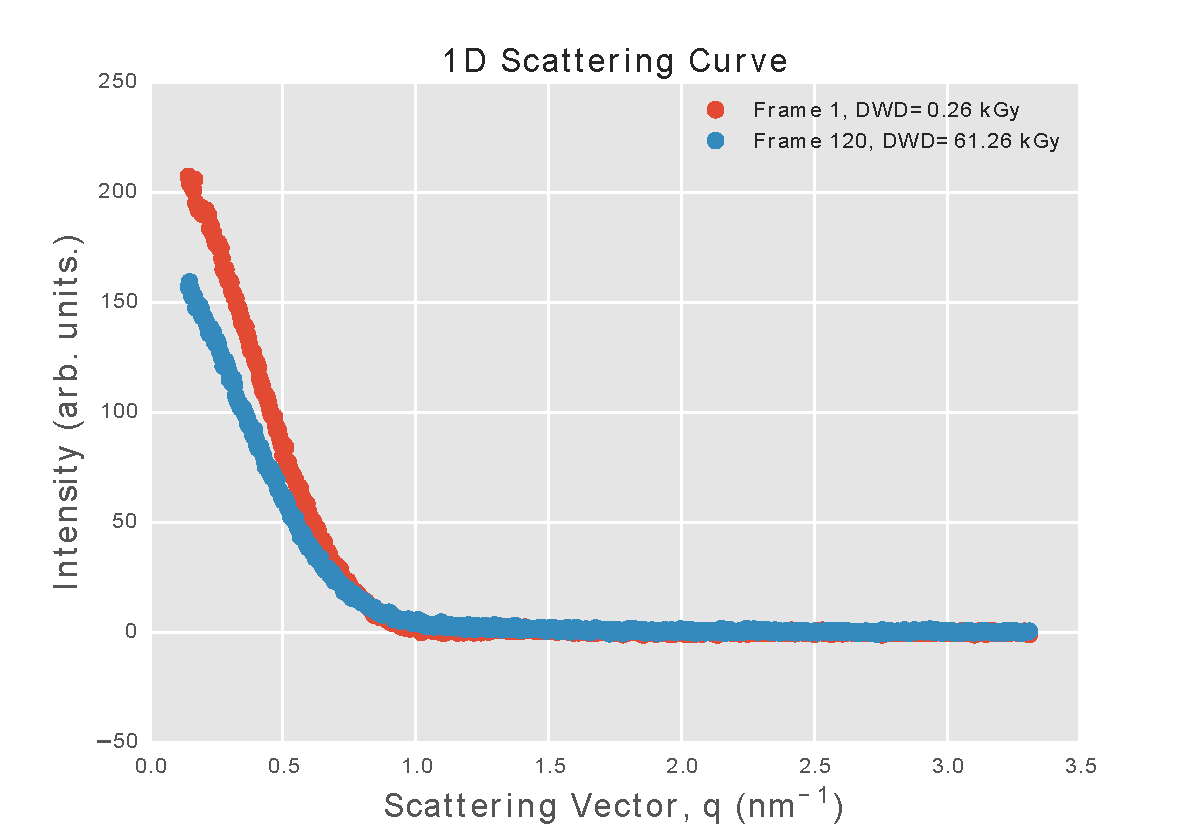
\includegraphics[width=\textwidth]{figures/saxs/scatter_curve_frames_1_120_amended.pdf}
            \caption{}
            \label{fig:1D scatter plot of frames 1 and 120}
    \end{subfigure}
    \\
    \begin{subfigure}[b]{0.9\textwidth}
            \centering
            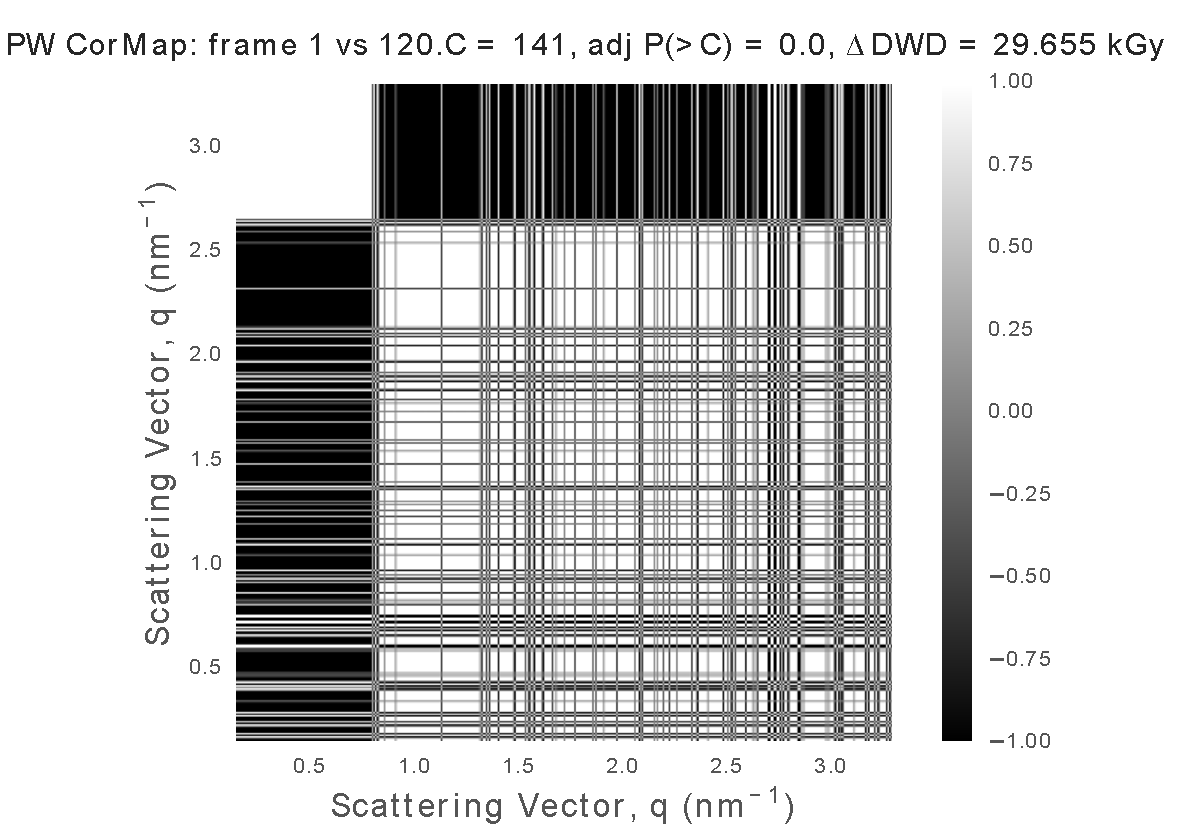
\includegraphics[width=\textwidth]{figures/saxs/pwcormap_frames_1_120_amended.pdf}
            \caption{}
            \label{fig:Pairwise correlation frames 1 and 120}
    \end{subfigure}
    \caption[Similarity comparison with selected frames from the first experimental repeat with no radioprotectant added]{Similarity comparison with selected frames from the first experimental repeat with no radioprotectant added. (a) 1D scatter curves for frames 1 and 2. These two curves overlap well and are classed as similar (b) Pairwise CorMap between frames 1 and 2. The ostensibly randomised lattice pattern suggests that the 1D curves are similar. (c) 1D scatter curves for frames 1 and 120. It is clear that these frames do not overlap. (d) Pairwise CorMap between frames 1 and 120. The dissimilarity between the two frames is represented by the large black and white regions.}
    \label{fig:Pairwise correlation plots}
\end{figure}

The problem can be thought of in an identical manner to a coin toss experiment with the following two conditions:
\begin{enumerate}
    \item the probability of the difference of any two data points being either positive or negative is 0.5,
    \item the result of the difference of any two data points with another two are assumed independent,
\end{enumerate}
In the coin toss experiment one can ask: `what is the probability of observing more than $n$ consecutive heads (or tails)?'.
The Schilling distribution \cite{schilling1990longest} calculates this probability.
For the SAXS experiment this is the same as asking for the probability of observing a patch of white (+1) or black (-1) larger than the longest patch of white or black that was actually observed in the pairwise CorMap.
More formally, we ask for the probability ($P$ value) of obtaining an edge length larger than $C$ (denoted $P(>C)$) within an $n$-by-$n$ correlation matrix.
This is calculated from the Schilling distribution with parameters $n$ and $C$.
If the $p$ value is smaller than a threshold value $\alpha$ ($\alpha \le$ 0.01 is recommended \cite{franke2015correlation}) then the two frames can be considered dissimilar.

The CorMap test is implemented in the current distribution of DATCMP, although the software does not include visualisation tools.
Since multiple pairwise tests have to be made from several comparisons, the Bonferroni correction\footnote{If multiple hypotheses are tested then the likelihood of observing a rare event (and thus the likelihood of incorrectly rejecting the null hypothesis) is increased. The Bonferroni correction, divides the overall statistical significance level, $\alpha$, by the number of tests, $n$, so that the hypotheses are tested individually at a significance level of $\alpha/n$.} is applied to the $P(>C)$ values resulting in $P_{adj}(>C)$ values.
The raw output from the program is essentially a list of $P(>C)$ and $P_{adj}(>C)$ values for all possible pairwise comparisons.
The set of $P_{adj}(>C)$ values that result from comparing the first frame to all subsequent frames is shown in Figure~\ref{fig:p values for comparisons with frame 1}.
\begin{figure}
    \centering
    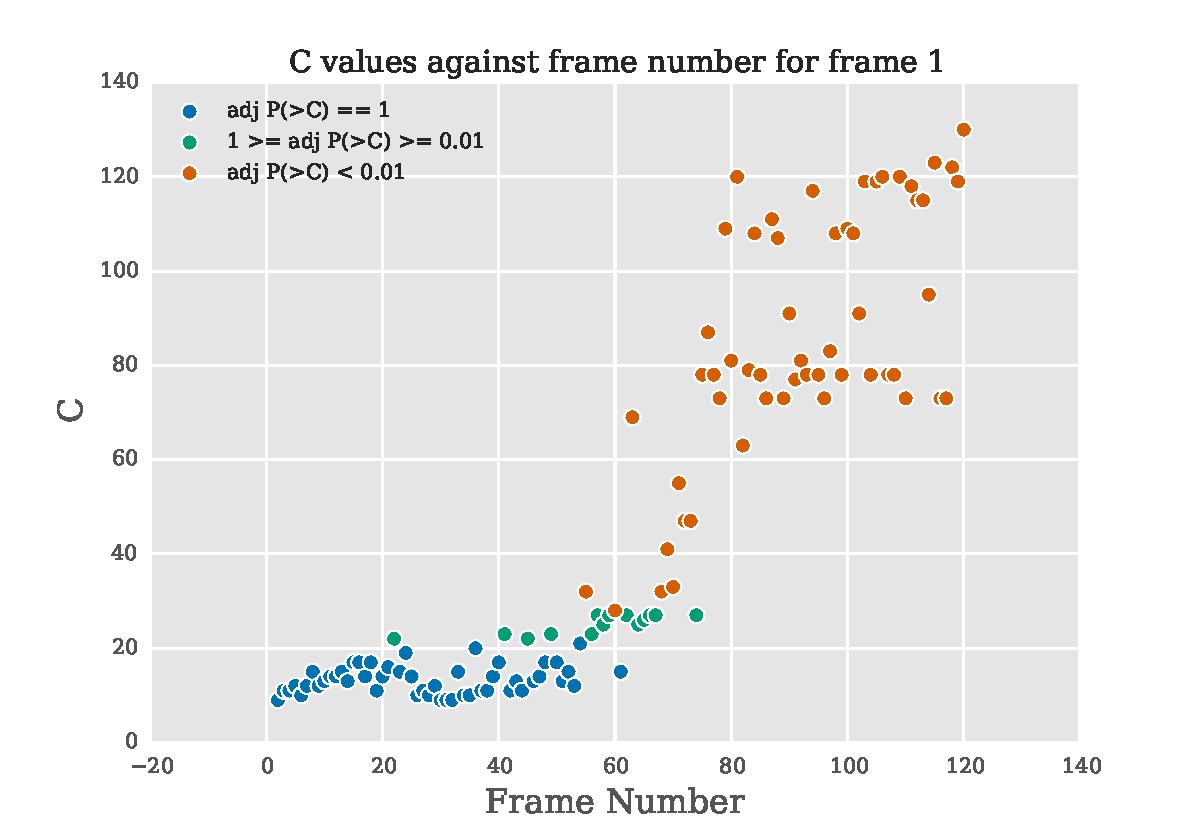
\includegraphics[width=1.0\textwidth]{figures/saxs/scatter_asc_10.pdf}
    \caption[Longest observed edge length against the frame number for pairwise comparisons with frame 1.]{Longest observed edge length $C$ against the frame number for pairwise comparisons with frame 1.
    For similar frames to frame 1, the pairwise CorMaps are more like randomised lattices (Figure~\ref{fig:Pairwise correlation frames 1 and 2}) and hence $C$ is fairly small.
    Therefore the chance of observing a longer edge length than $C$ is high ($P_{adj}(>C) = 1$ - blue circles).
    As frames start becoming more dissimilar, the $C$ values increase and the $P_{adj}(>C)$ values fall.
    These circles are coloured green.
    When frames are very dissimilar, $C$ becomes very large (Figure~\ref{fig:Pairwise correlation frames 1 and 120}) and $P_{adj}(>C) <$ 0.01.
    The circles representing the comparison with these frames are coloured orange.
    The first dissimilar frame (coloured orange - frame 55) is may not necessarily be the point at which frames should stop being merged according to this analysis, because there are circles after frame 55 that are not orange in colour.}
    \label{fig:p values for comparisons with frame 1}
\end{figure}

\subsubsection{Applying this methodology to Expt 2 results}
\label{subs:Applying this methodology to Expt 2 results}
As can be seen in Figure~\ref{fig:p values for comparisons with frame 1}, the first frame which is calculated to be dissimilar to frame 1 is frame 55 (first orange circle) which has a corresponding dose of 14.73$\,$kGy.
Therefore the threshold for radiation damage onset to be significant could be set at that frame.
However the frames immediately after 55 do not have $P_{adj}(>C) <$ 0.01 (green or blue circles) suggesting that these frames are not significantly dissimilar to frame 1.
Thus frame 55 may be a noisy outlier and radiation damage may not necessarily be significant at that frame.
A more robust check may be to find the first dissimilar frame for which $m$ consecutive frames are dissimilar.
This possibility was thus investigated and tested for $m$ = 1, 3, 5, 7 and 10 to determine the value $m = m_0$ for which $m > m_0$ did not significantly change the dose at which frames were determined to be dissimilar.
Figure~\ref{fig:Num consecutive frame test} shows the result of the test for all of the radioprotectant experiments (note that the dose is used as the threshold for radiation damage instead of frame number).
\begin{figure}
    \centering
    \begin{subfigure}[b]{0.75\textwidth}
            \centering
            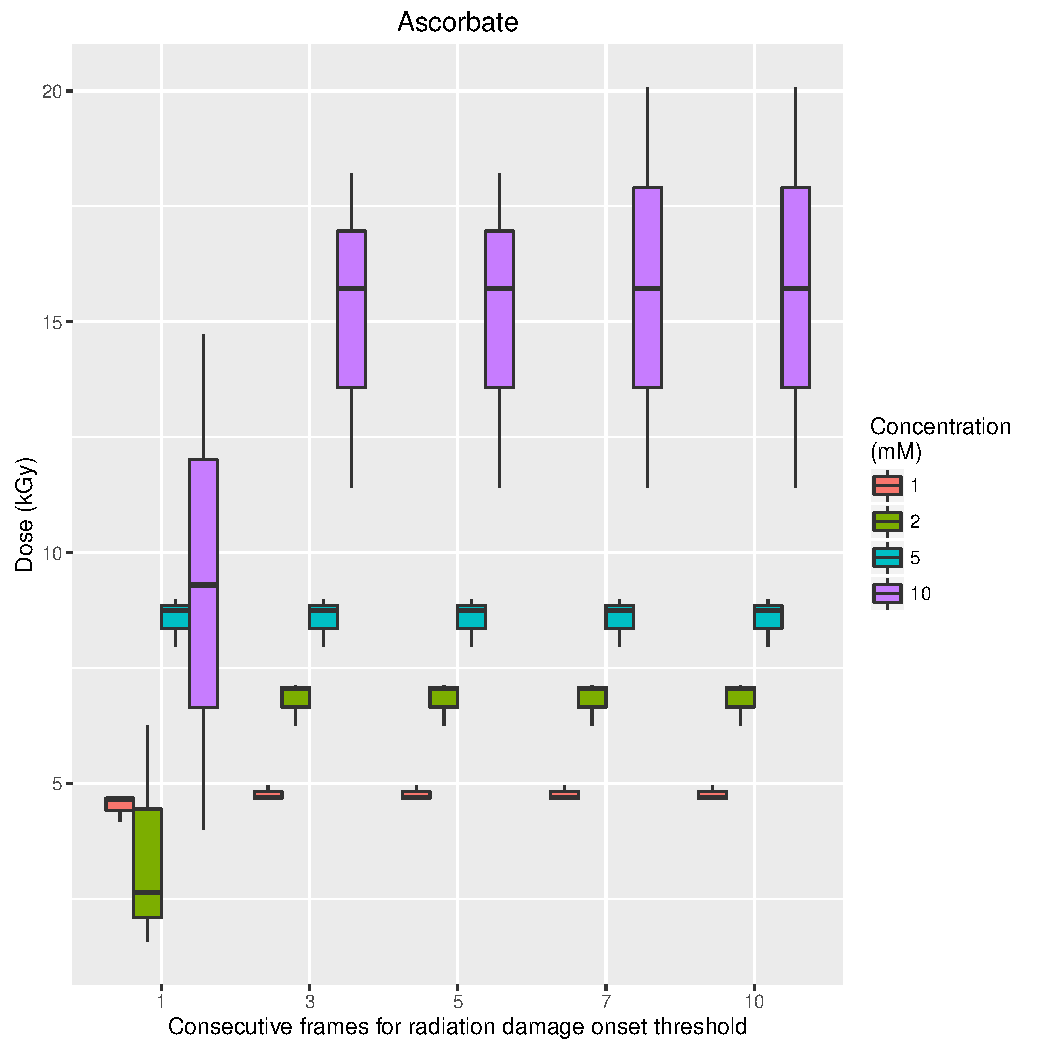
\includegraphics[width=\textwidth]{figures/saxs/Ascorbate_Num_consec_fr_comp.pdf}
            \caption{}
            \label{}
    \end{subfigure}
    \\
    \begin{subfigure}[b]{0.75\textwidth}
            \centering
            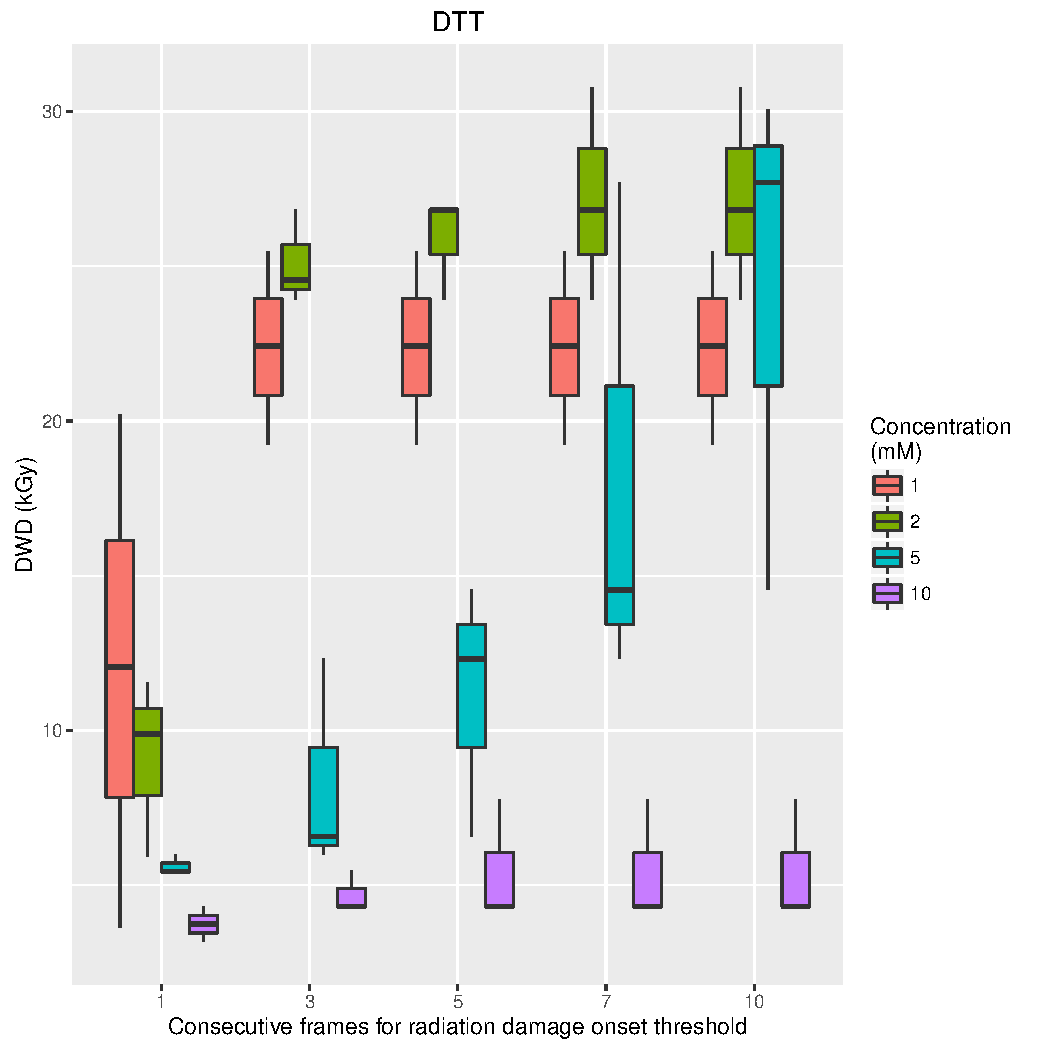
\includegraphics[width=\textwidth]{figures/saxs/DTT_Num_consec_fr_comp.pdf}
            \caption{}
            \label{fig:Num consec frames - DTT}
    \end{subfigure}
\end{figure}
\begin{figure}
    \ContinuedFloat
    \centering
    \begin{subfigure}[b]{0.75\textwidth}
            \centering
            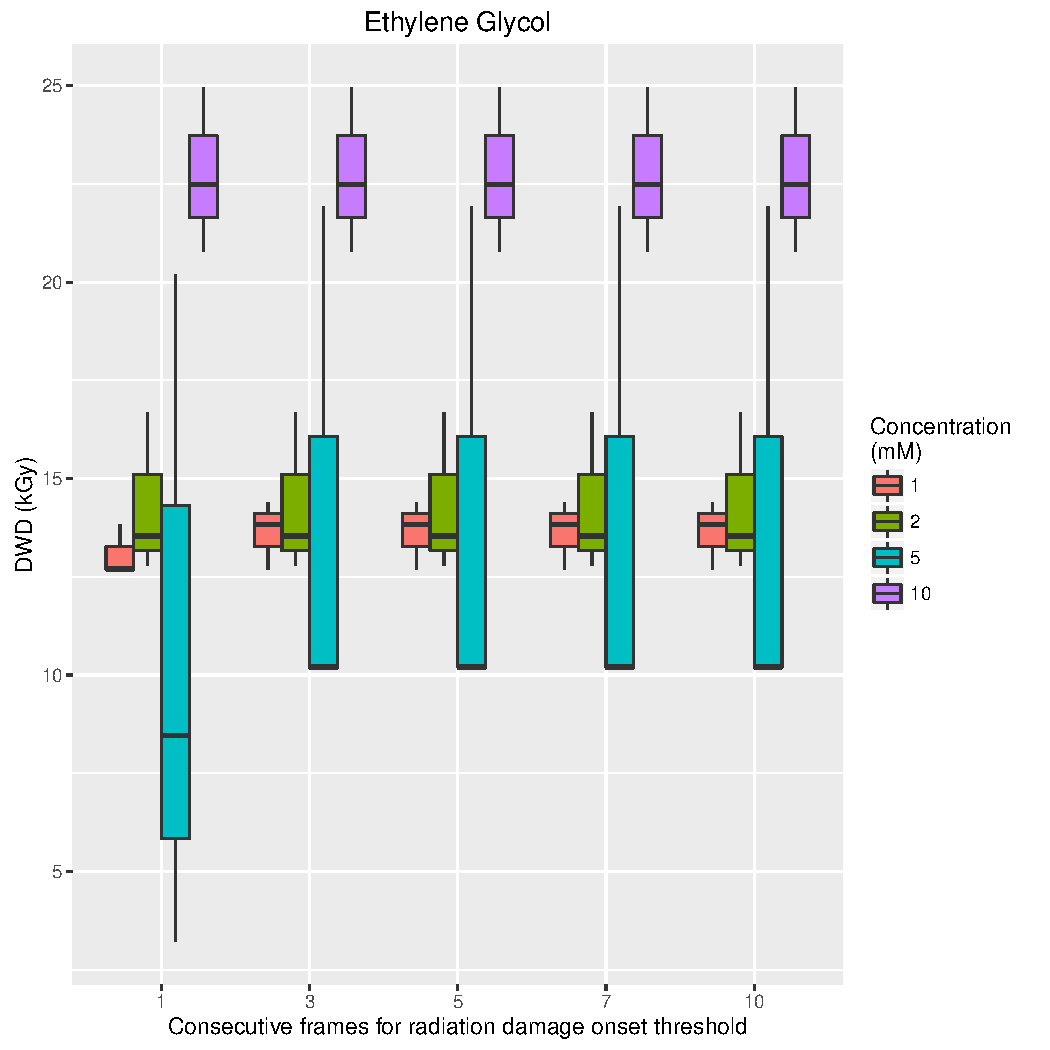
\includegraphics[width=\textwidth]{figures/saxs/Ethylene_Glycol_Num_consec_fr_comp.pdf}
            \caption{}
            \label{}
    \end{subfigure}
    \\
    \begin{subfigure}[b]{0.75\textwidth}
            \centering
            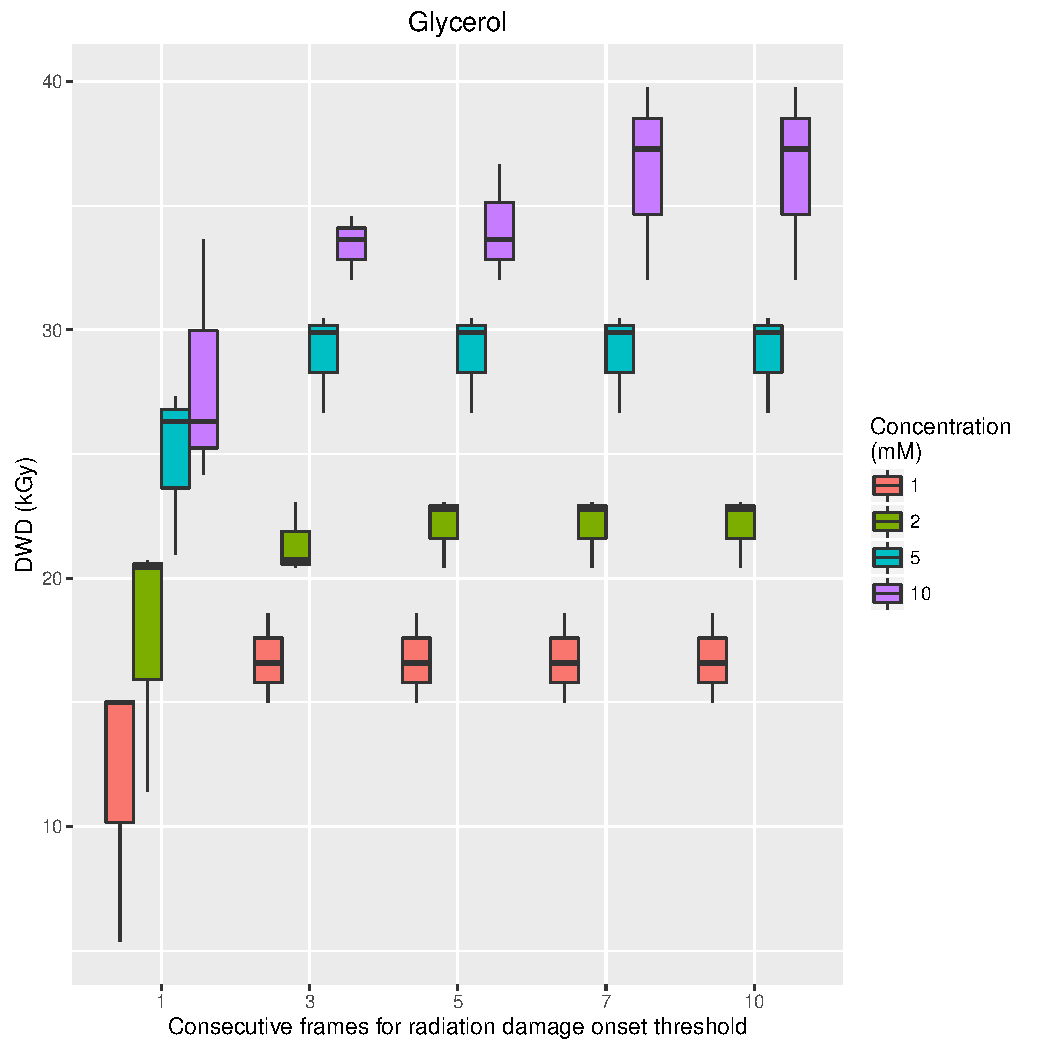
\includegraphics[width=\textwidth]{figures/saxs/Glycerol_Num_consec_fr_comp.pdf}
            \caption{}
            \label{}
    \end{subfigure}
\end{figure}
\begin{figure}
    \ContinuedFloat
    \centering
    \begin{subfigure}[b]{0.75\textwidth}
            \centering
            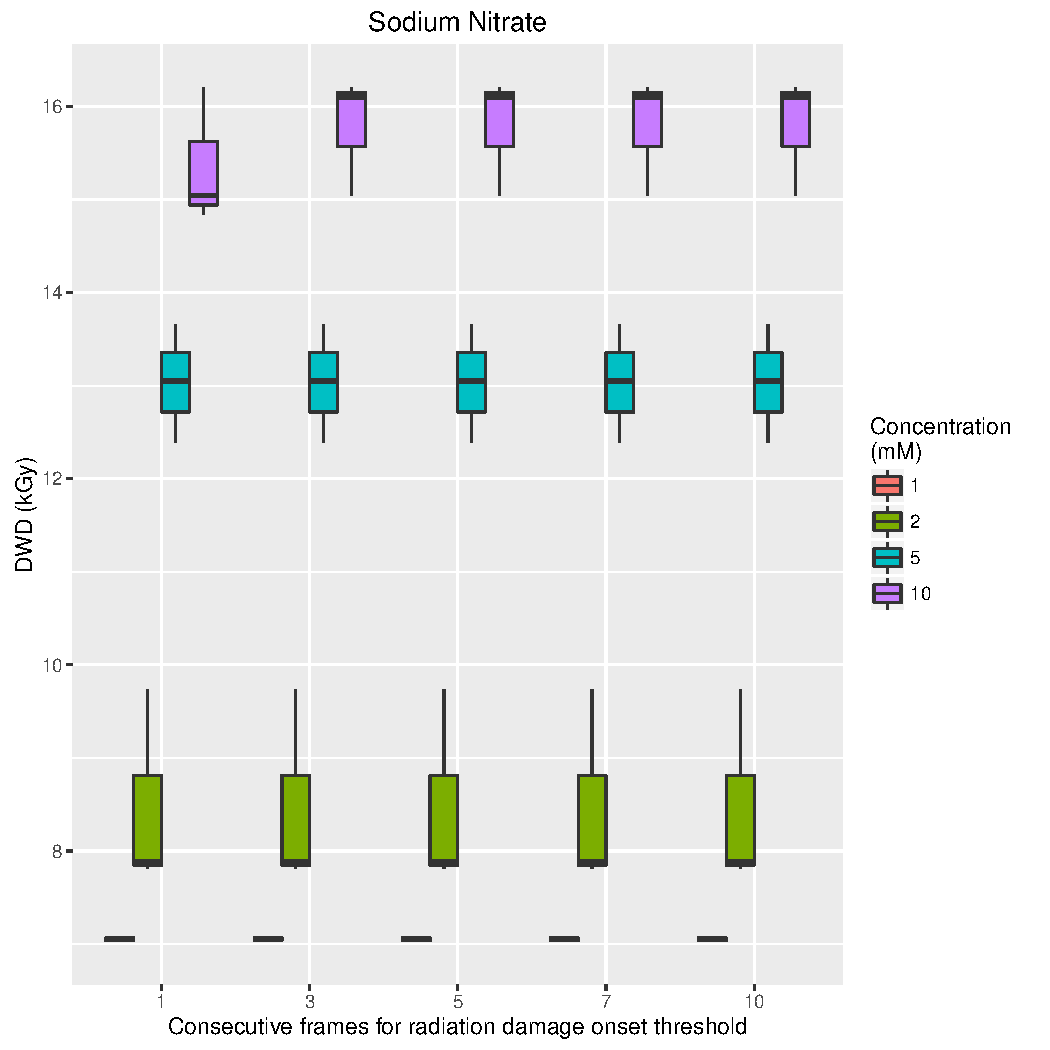
\includegraphics[width=\textwidth]{figures/saxs/Sodium_Nitrate_Num_consec_fr_comp.pdf}
            \caption{}
            \label{}
    \end{subfigure}
    \\
    \begin{subfigure}[b]{0.75\textwidth}
            \centering
            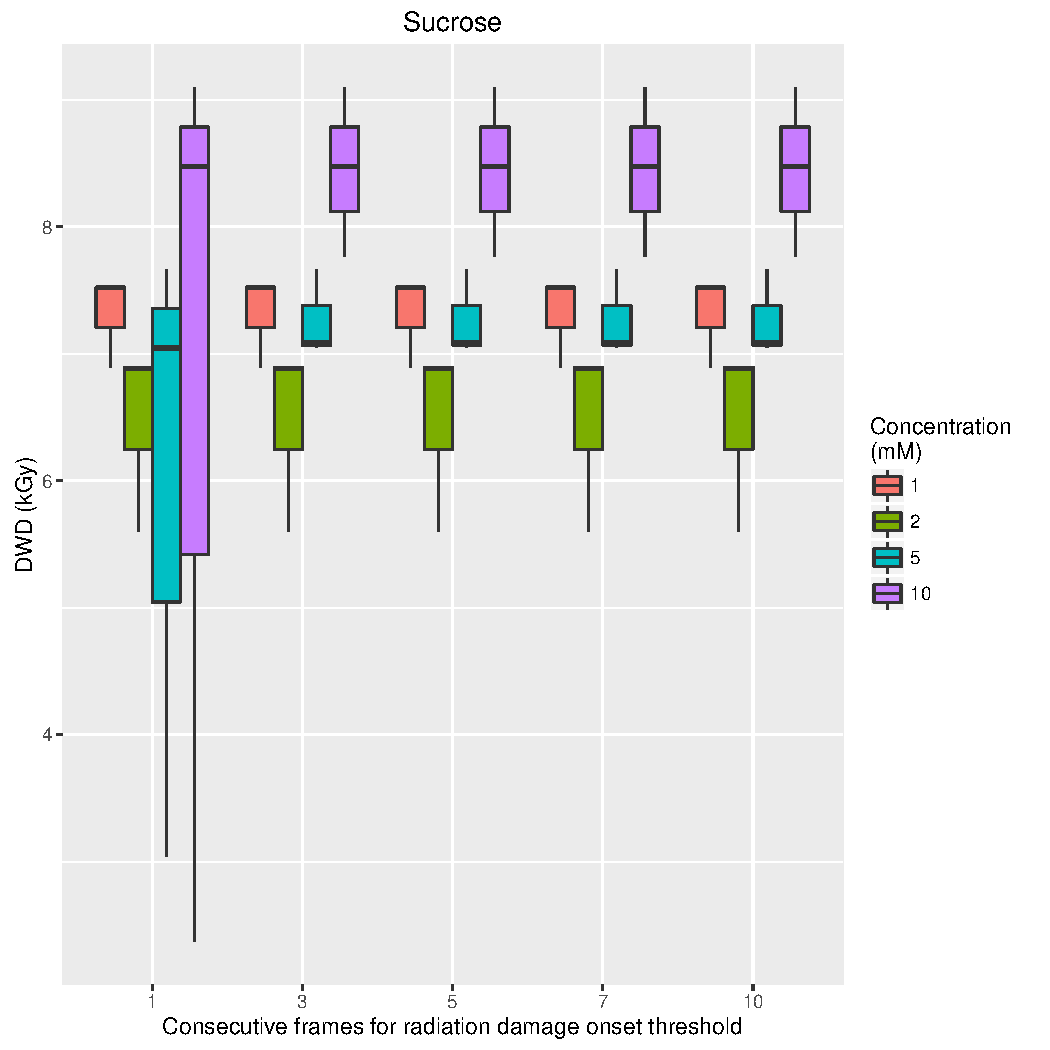
\includegraphics[width=\textwidth]{figures/saxs/Sucrose_Num_consec_fr_comp.pdf}
            \caption{}
            \label{}
    \end{subfigure}
\end{figure}
\begin{figure}
    \ContinuedFloat
    \centering
    \begin{subfigure}[b]{0.75\textwidth}
            \centering
            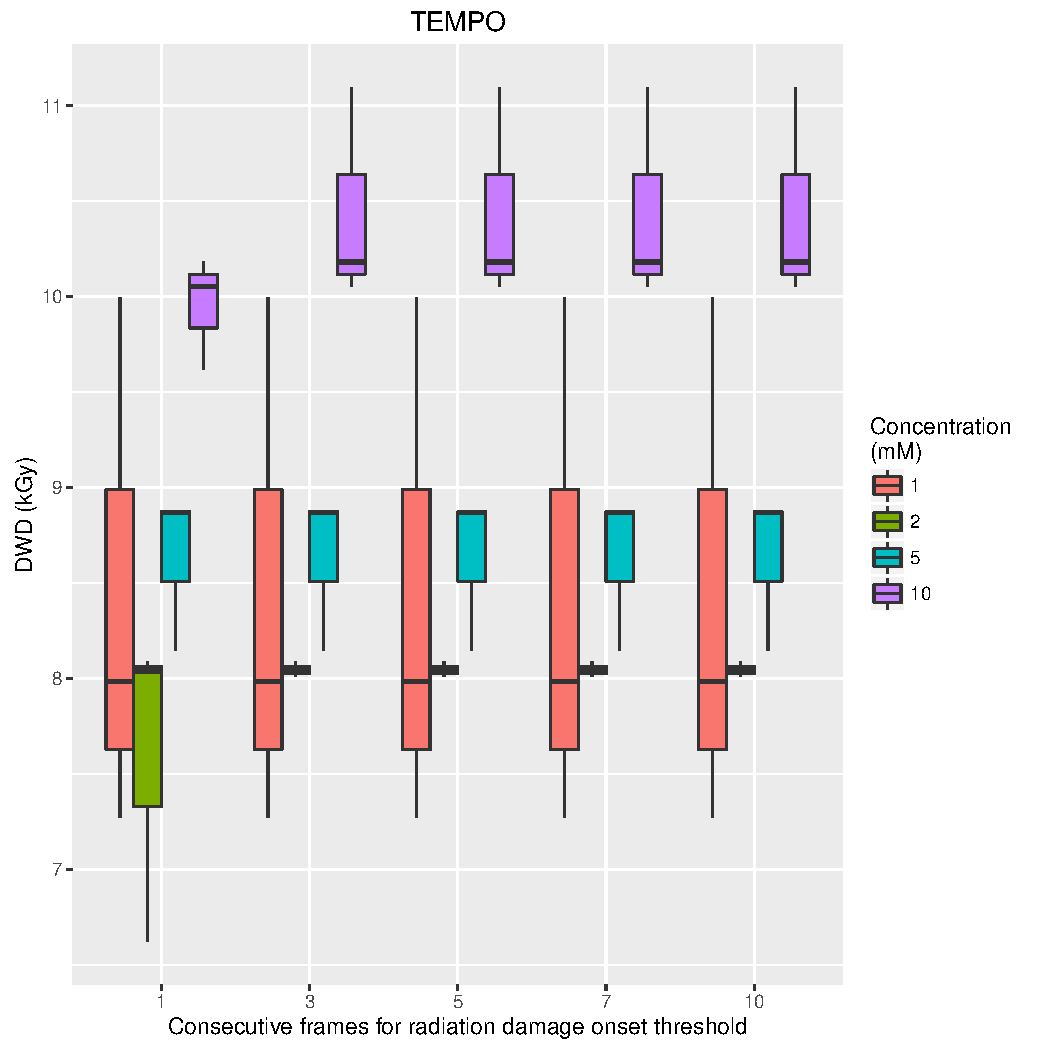
\includegraphics[width=\textwidth]{figures/saxs/TEMPO_Num_consec_fr_comp.pdf}
            \caption{}
            \label{}
    \end{subfigure}
    \\
    \begin{subfigure}[b]{0.75\textwidth}
            \centering
            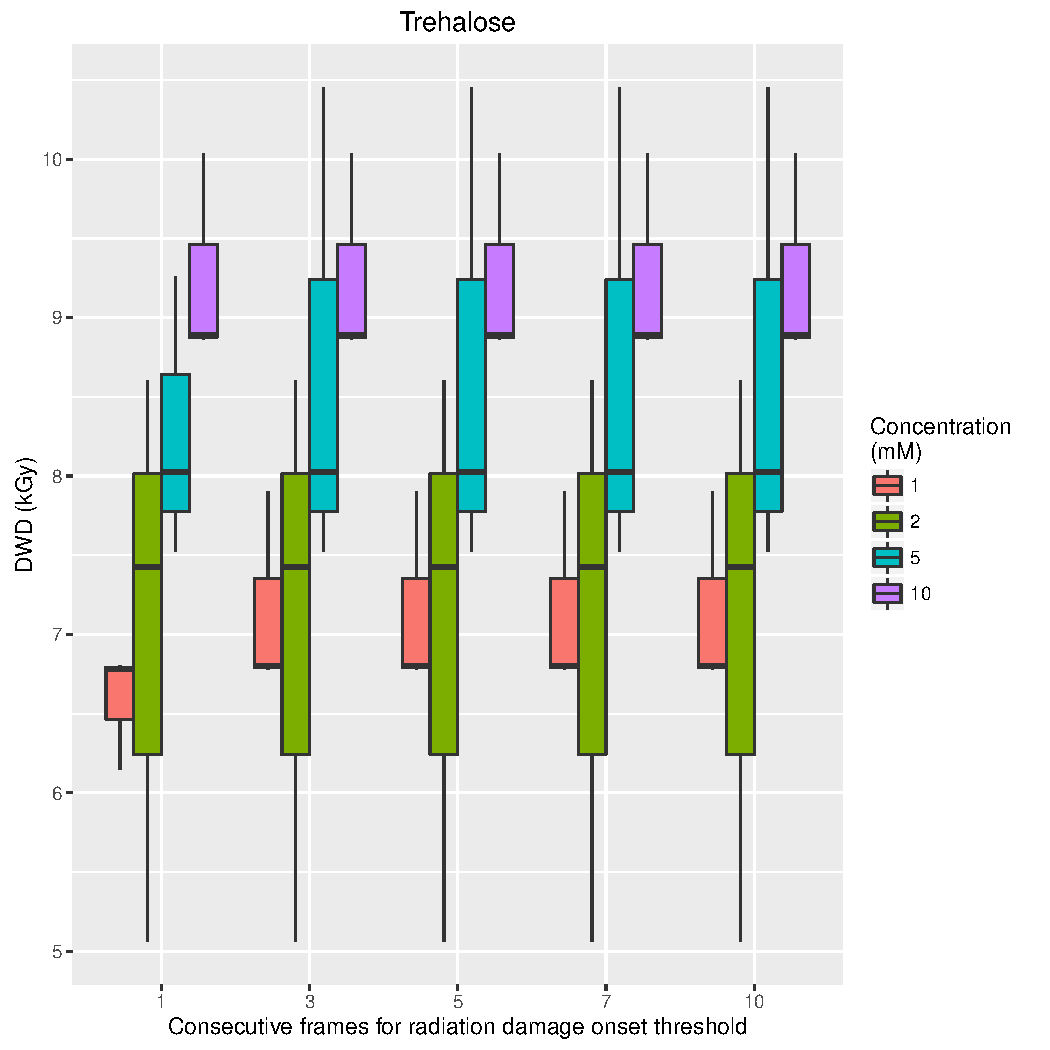
\includegraphics[width=\textwidth]{figures/saxs/Trehalose_Num_consec_fr_comp.pdf}
            \caption{}
            \label{}
    \end{subfigure}
    \caption[Dose at which significant radiation damage is determined to have occurred for different values of $m$, the number of consecutive dissimilar frames.]{Dose at which significant radiation damage is determined to have occurred for different values of $m$, the number of consecutive dissimilar frames, for the 8 radioprotectants tested in Expt 2.}
    \label{fig:Num consecutive frame test}
\end{figure}
It can be seen that for most radio protectant compounds if $m$ = 1, the spread of the apparent radiation damage onset is generally larger than for $m$ = 3, 5, 7, 10.
For $m$ = 3, 5, 7, 10 the values corresponding to the onset of significant radiation damage are practically identical (except for DTT, but this is dealt with in section \ref{sub:Experiment 2 - Results}).
Thus for the subsequent radiation damage analysis, the comparisons were performed with $m$ = 3.

The other parameter that may affect the conclusions of this method for radiation damage analysis is the threshold level $\alpha$. Therefore three different thresholds were set, $\alpha$ = 0.01, 0.05 and 0.1.
Figure~\ref{fig:alpha threshold value test} shows the result of this test with all of the radioprotectant data.
\begin{figure}
    \centering
    \begin{subfigure}[b]{0.75\textwidth}
            \centering
            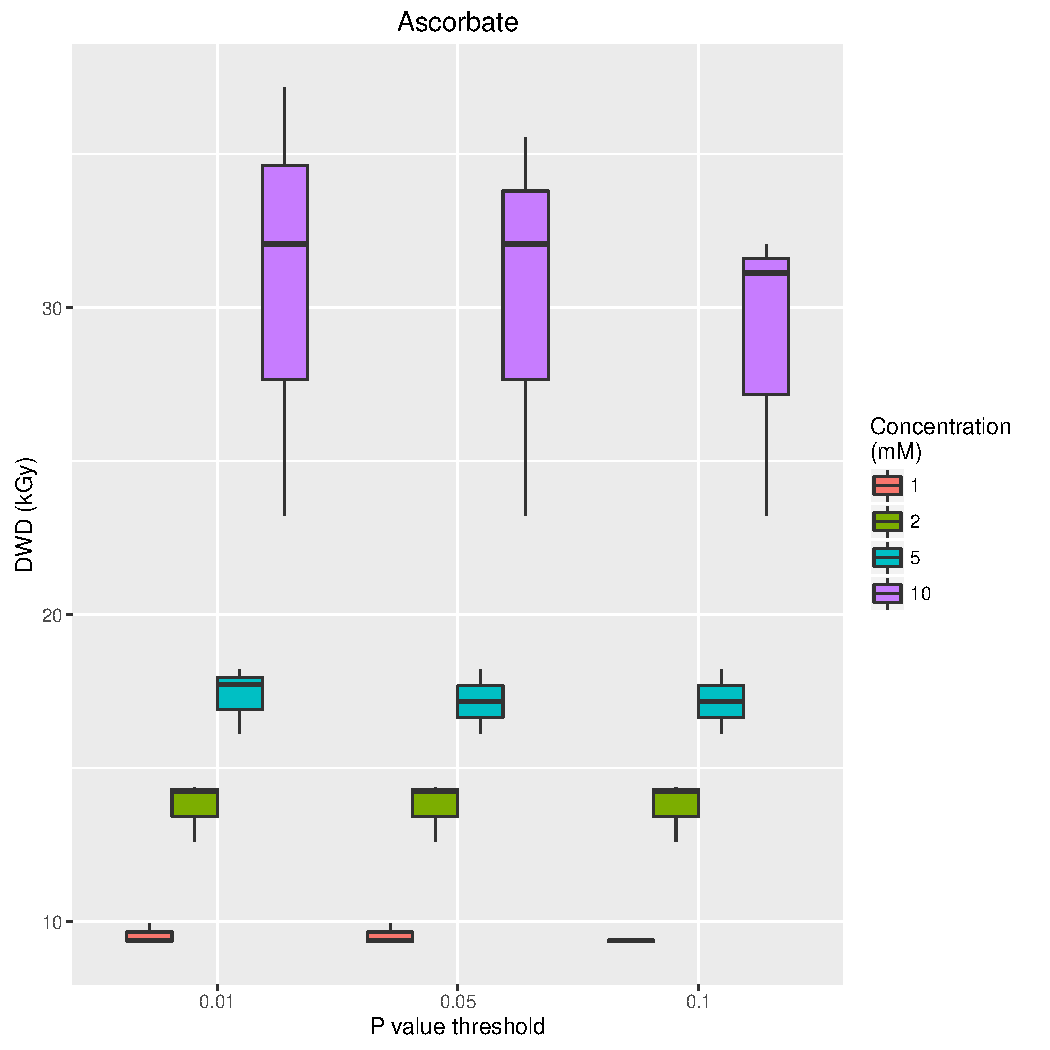
\includegraphics[width=\textwidth]{figures/saxs/Ascorbate_PThresh_comp.pdf}
            \caption{}
            \label{}
    \end{subfigure}
    \\
    \begin{subfigure}[b]{0.75\textwidth}
            \centering
            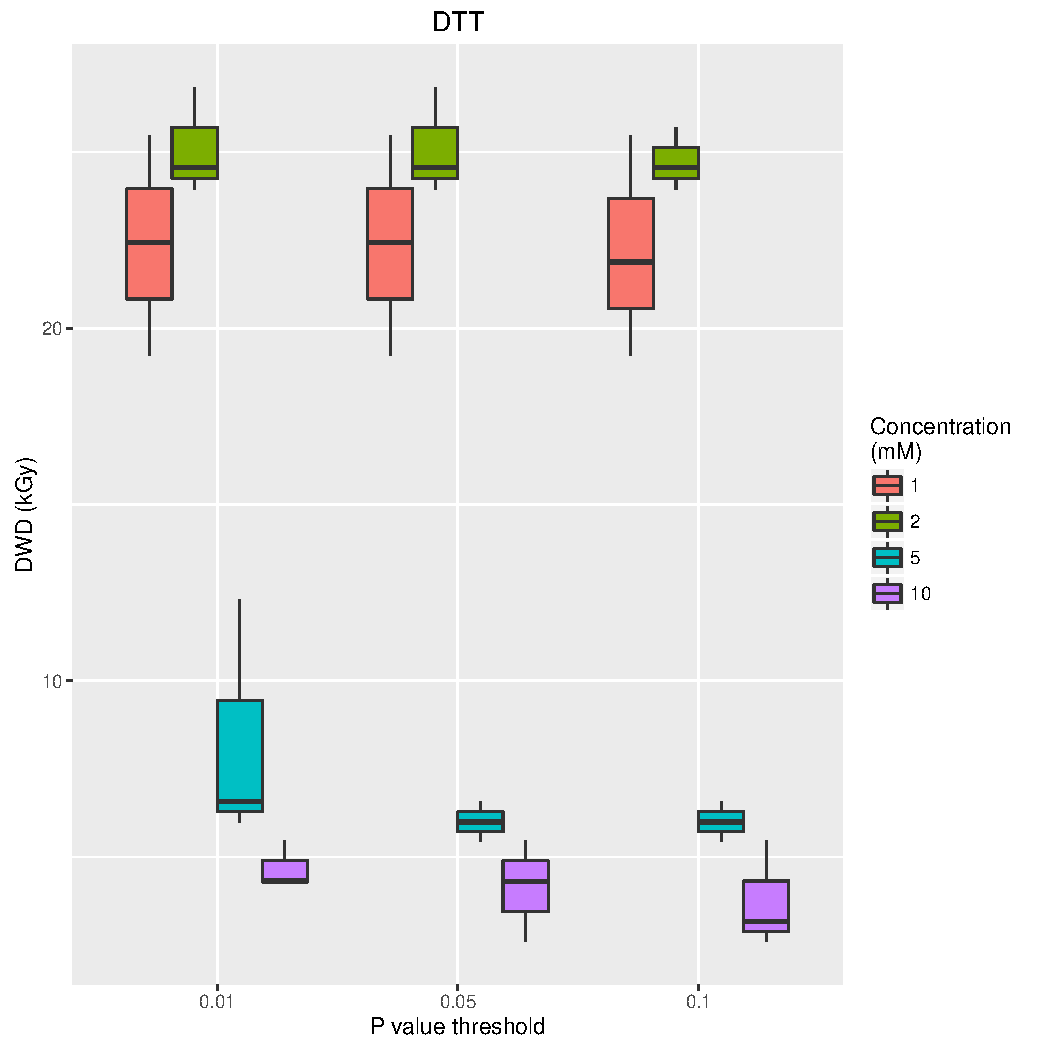
\includegraphics[width=\textwidth]{figures/saxs/DTT_PThresh_comp.pdf}
            \caption{}
            \label{}
    \end{subfigure}
\end{figure}
\begin{figure}
    \ContinuedFloat
    \centering
    \begin{subfigure}[b]{0.75\textwidth}
            \centering
            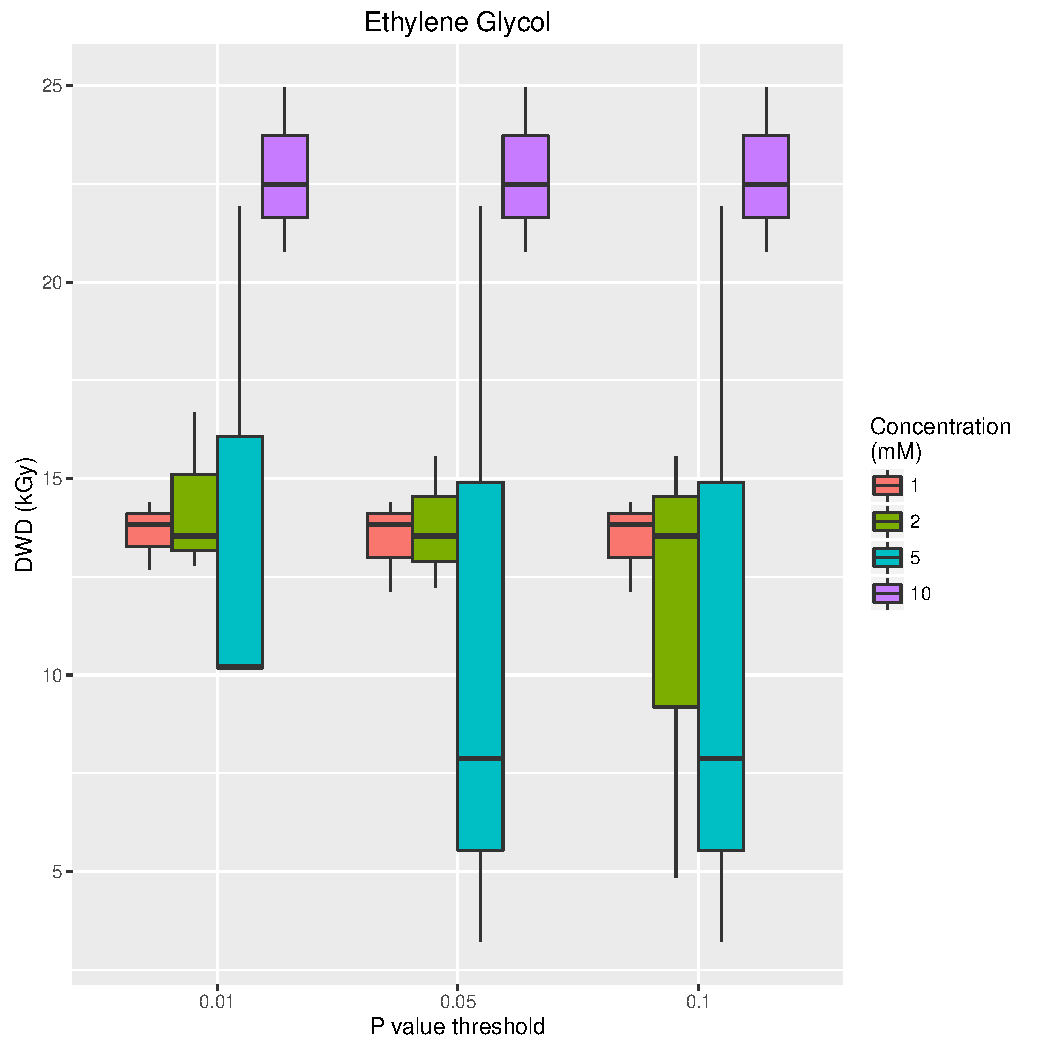
\includegraphics[width=\textwidth]{figures/saxs/Ethylene_Glycol_PThresh_comp.pdf}
            \caption{}
            \label{}
    \end{subfigure}
    \\
    \begin{subfigure}[b]{0.75\textwidth}
            \centering
            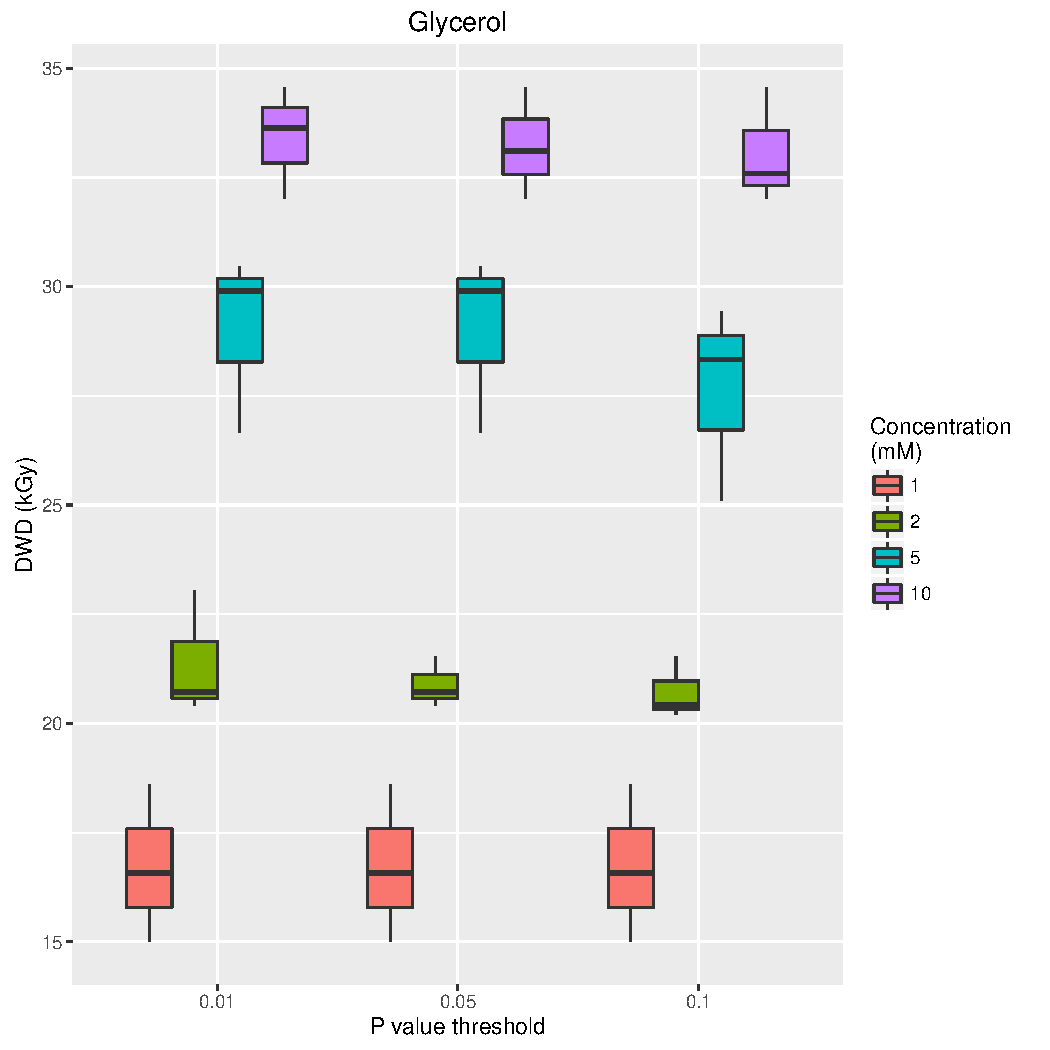
\includegraphics[width=\textwidth]{figures/saxs/Glycerol_PThresh_comp.pdf}
            \caption{}
            \label{}
    \end{subfigure}
\end{figure}
\begin{figure}
    \ContinuedFloat
    \centering
    \begin{subfigure}[b]{0.75\textwidth}
            \centering
            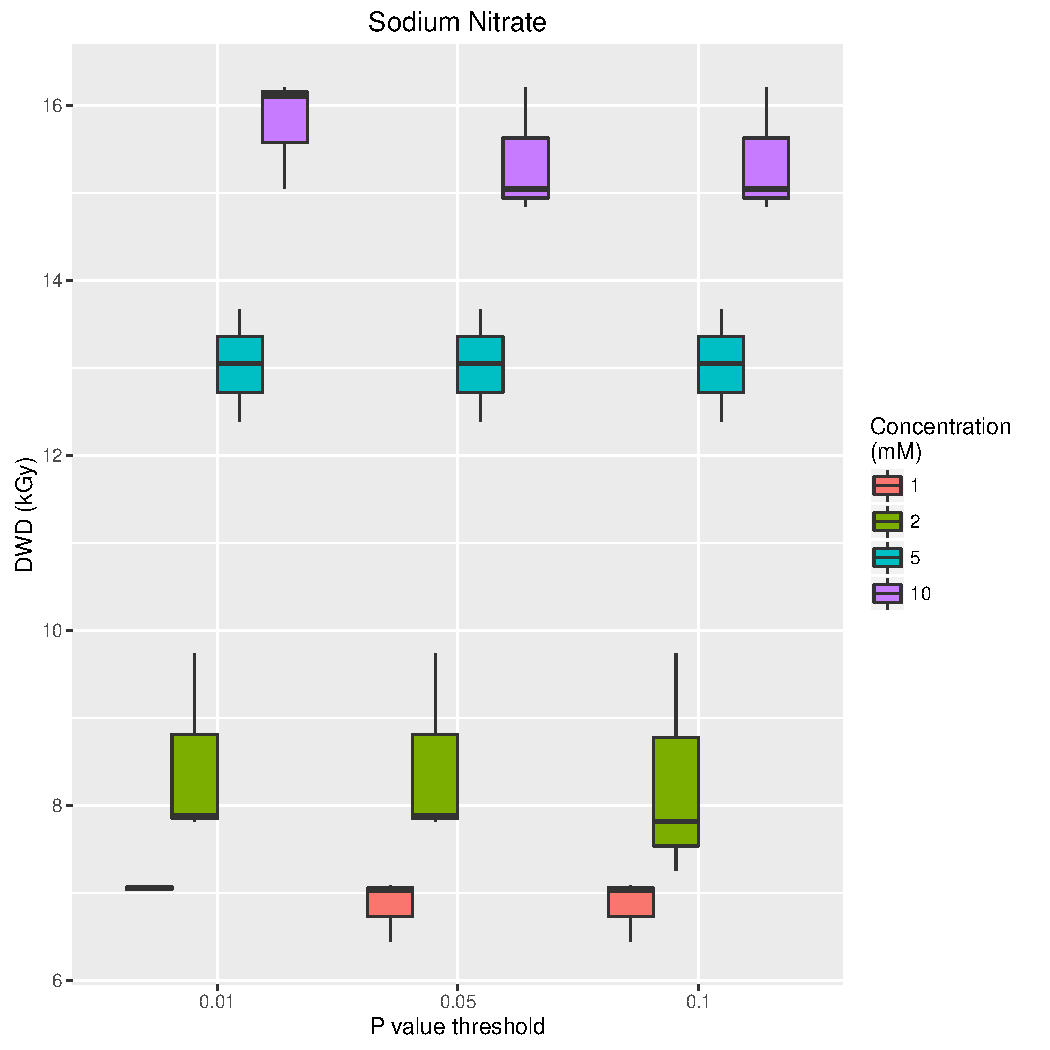
\includegraphics[width=\textwidth]{figures/saxs/Sodium_Nitrate_PThresh_comp.pdf}
            \caption{}
            \label{}
    \end{subfigure}
    \\
    \begin{subfigure}[b]{0.75\textwidth}
            \centering
            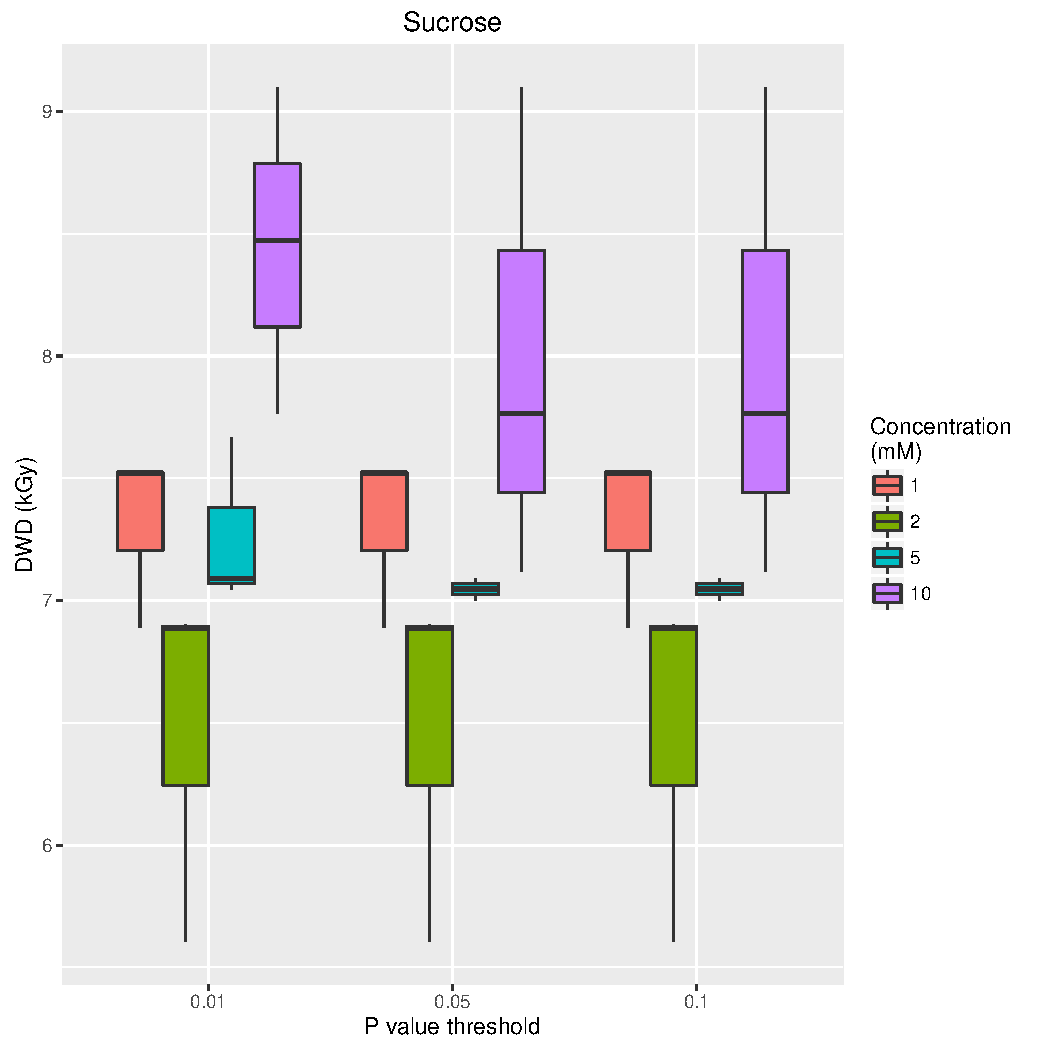
\includegraphics[width=\textwidth]{figures/saxs/Sucrose_PThresh_comp.pdf}
            \caption{}
            \label{}
    \end{subfigure}
\end{figure}
\begin{figure}
    \ContinuedFloat
    \centering
    \begin{subfigure}[b]{0.75\textwidth}
            \centering
            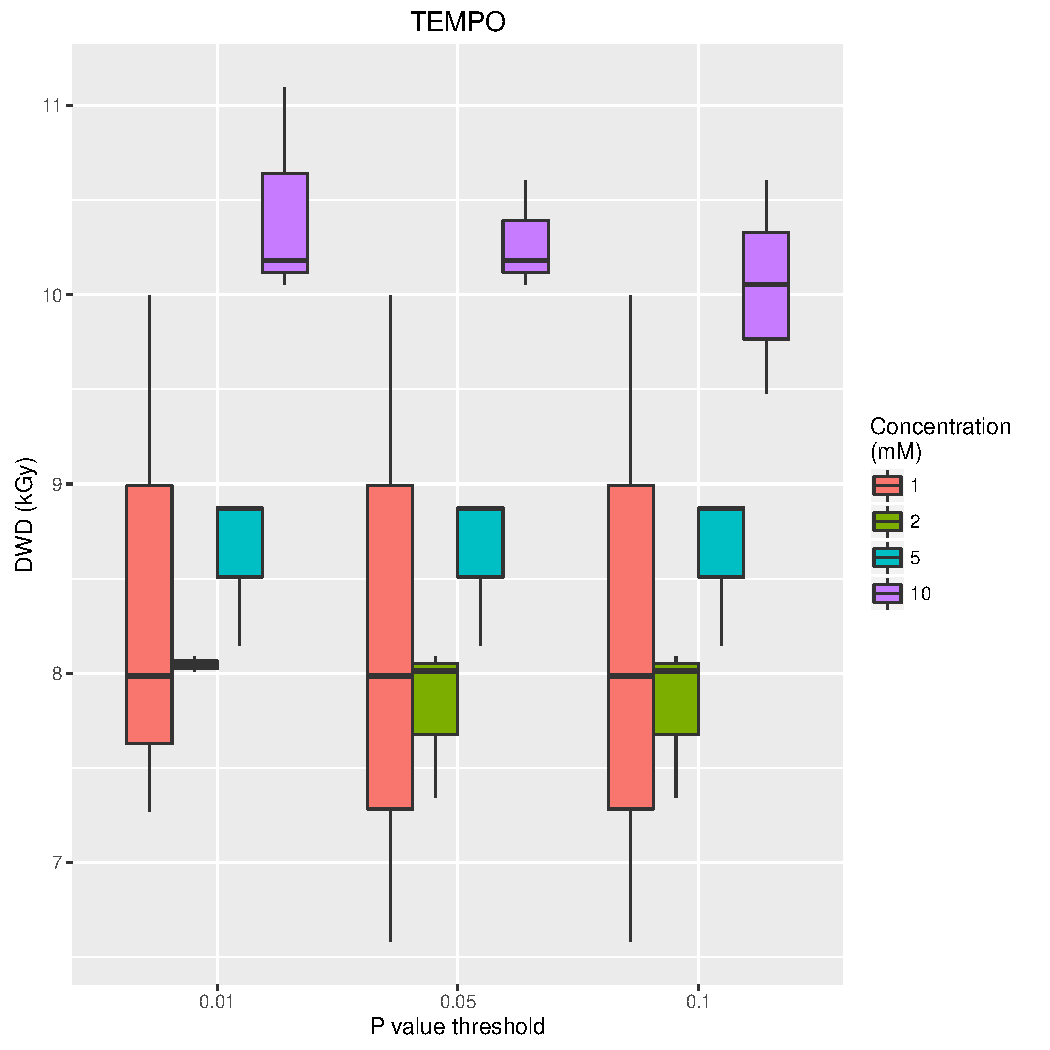
\includegraphics[width=\textwidth]{figures/saxs/TEMPO_PThresh_comp.pdf}
            \caption{}
            \label{}
    \end{subfigure}
    \\
    \begin{subfigure}[b]{0.75\textwidth}
            \centering
            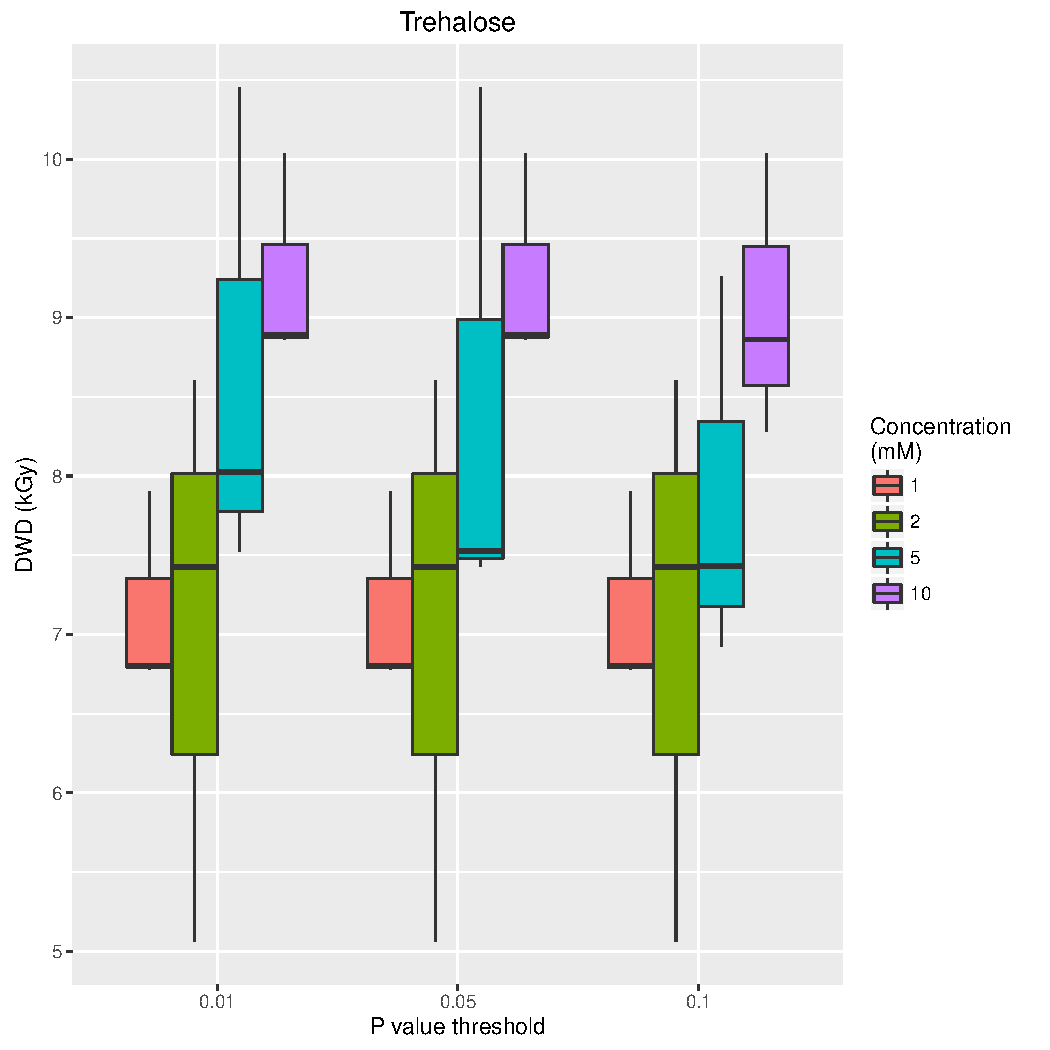
\includegraphics[width=\textwidth]{figures/saxs/Trehalose_PThresh_comp.pdf}
            \caption{}
            \label{}
    \end{subfigure}
    \caption[Dose at which significant radiation damage is determined to have occurred for different values of $\alpha$, the threshold probability value to determine frame similarity.]{Dose at which significant radiation damage is determined to have occurred for different values of $\alpha$, the threshold probability value to determine frame similarity, for the 8 radioprotectants tested in Expt 2.}
    \label{fig:alpha threshold value test}
\end{figure}
It can be seen that the median values are very similar for the various $\alpha$ values.
Given this fact and that $\alpha$ = 0.01 is the recommended (and sufficiently strict) threshold \cite{franke2015correlation}, $\alpha$ = 0.01 was chosen as the value used for all radioprotectant compounds in the subsequent radiation damage analysis.
The advantage of using $\alpha$ = 0.01 is that frames have to be very dissimilar before the $P_{adj}(>C)$ value falls below that value.
This means that it is less likely that frames are discarded when they actually are similar (in statistical speak this means there is less chance of a type I error).
